\section{Requirements and System Model}\label{sec:requirements}
Big data is highly dependent on cloud-edge computing, which makes extensive use of multitenancy.
Multitenancy permits sharing one instance of infrastructures, platforms or applications by multiple tenants to optimize costs. This leads to common scenarios where a service provider offers subscription-based analytics capabilities in the cloud, or a single data lake is accessed by multiple customers. Thus, it is a common situation to have a big data pipeline where data and services belong to various organizations, posing a serious risk of potential privacy and security violation.
\hl{NON CHIARISSIMA The fundamental concept underlying our methodology is to enhance the prevailing paradigm for big data pipelines through the creation of a data governance framework tailored to contemporary data-driven pipelines.} The primary objective of this framework is to facilitate the assembly of data processing services, with a central focus on the selection of these services to optimize data quality, while upholding privacy standards. In the following of this section,
we present our system model (Section \ref{sec:systemmodel}) and our reference scenario (Section \ref{sec:reference}).

\subsection{System Model}\label{sec:systemmodel}
Our guiding principle is to balance two critical requirements: data quality and data privacy. In today's data landscape, the coexistence of data quality and data privacy is critical. The increase in data production has led to a split in scientific research priorities. This has resulted in two main focus areas. First, researchers are exploring methods to optimize valuable data. Here, ensuring data quality is vital, and requires accuracy, reliability, and suitability for analytical purposes.
Second, there is a need to prioritize data privacy and security. This involves safeguarding confidential information and complying with strict privacy regulations. These two directions are happening at the same time, but there are not many solutions that find a good balance between them.
Our approach seeks to harmonize these objectives by establishing a framework that balances privacy and data quality.

Our system model is composed by the following parties:
\begin{description}
  \item[User] that wants to perform some analytics on the data;
  \item[Pipeline], the sequence of connected services that collect, prepare, process, and analyze data  in a structured and automated manner. We distinguish between a pipeline template that acts as a skeleton, specifying the structure of the pipeline and the (non-)functional requirements driving  service selection, and a pipeline instance instantiating the template with services according to the specified requirements;
  \item[Service], a software that performs a specific task according to specific access control privileges on data; %, a service can be tagged with some policies %, a service is characterized by two function: the service function and the policy function.
  \item[Data Governance Policy], a structured set of confidentiality guidelines, rules, and procedures that define how and when the service can access ad must safeguard data;
\end{description}


In our context, an \user aims to execute a data pipeline to perform analysis or transformation procedures on some data.
The input data are assumed to be ready for analysis, that is, they underwent a preparatory phase that addressed issues such as missing values, outliers, and formatting discrepancies, ensuring that the data are in an optimal state for subsequent analysis.
% Policies governing the data are established, which can originate from the \user, third-party entities, or regulatory frameworks.
% For instance, a policy may restrict the execution of processing operations to a specific geographic region.
The \user is presented with a list of pipeline templates. When the template is selected according to the \user\ requirements, \user\ is presented with a list of candidate services for each composite service in the template. We assume services to be functionally equivalent and comply with the privacy policies specified in the template.
Services are ranked based on their ability to retain the maximum amount of information while maintaining a level of privacy.
Priority is given to the service that maximizes data quality while maintaining the same level of privacy.
This evaluation process aids in identifying the most suitable service for a particular step in the pipeline.
Upon selecting the most suitable service for each step, the pipeline instantiation is considered complete and ready for execution.
It is important to emphasize that our goal is not to formulate novel service composition algorithms, but rather to establish a data governance framework.

It is important to note that our approach builds on the following assumption: \emph{upholding a larger quantity of data is linked to better data quality.} While this assumption is not true in all settings, it correctly represents many real-world scenarios. We leave a solution that departs from this assumption to our future work.

\subsection{Reference Scenario}\label{sec:reference}
Our reference scenario is a service-based environment where services are composed according to a pipeline template.
The case study is based on an analysis of a dataset consisting of individuals detained in Department of Correction facilities in the state of Connecticut while awaiting trial.
The dataset\footnote{https://data.ct.gov/Public-Safety/Accused-Pre-Trial-Inmates-in-Correctional-Faciliti/b674-jy6w} exhibits a straightforward row-and-column structure.
Each row represents an inmate; each columns include the following attributes: date of download, a unique identifier, last entry date, race, gender, age of the individual, the bound value, offense, entry facility, and detainer.
To serve the objectives of our study, we have extended this dataset by introducing randomly generated first and last names. 

We envision the establishment of a service pipeline designed as follows.
The end user, a member of the Connecticut Department of Correction (DOC), seeks to perform an analysis on the dataset to compare admission trends in Connecticut prisons with those in other states.
The user's preferences align with a predefined template that orchestrates the following sequence of operations: 
\emph{i)} Anonymization of the dataset.
\emph{ii)} Data enrichment, integrating data from the states of New York and New Hampshire.
\emph{iii)} Transformation of the dataset to derive state-specific data aggregations, including statistical measures like averages, medians, and clustering-based statistics.
\emph{iv)} Storage of the results in the corresponding states. Specifically, one copy remains in Connecticut (where sensitive information in the source dataset is not protected), while two additional copies are distributed to New York and New Hampshire (with sensitive information from the source dataset being safeguarded).

It should be noted that the template requires the execution of the entire service within a single country.
In cases where the data needs to be transmitted beyond the boundaries of Connecticut, data protection measures are implemented.
A visual representation of the flow is presented in Figure \ref{fig:service_composition_example}.

\begin{figure}
  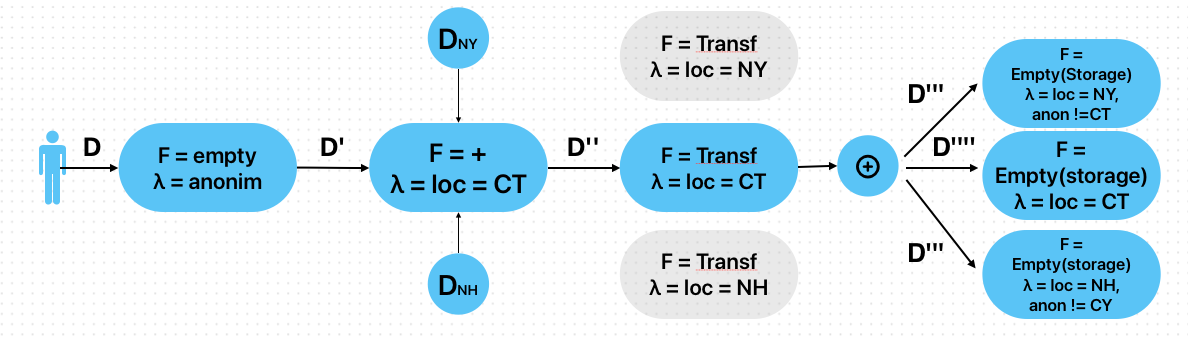
\includegraphics[width=0.98\columnwidth]{service_composition_example}
  \caption{Service composition example.}\label{fig:service_composition_example}

\end{figure}



